\chapter{Beginning Algebra}

\section{Intro}

This course covers 9th grade math, i.e. the first year of high school mathematics.

\section{The Three Forms of Linear Equations and Finding Slope}

% \vspace{1 cm}

% \centerline{\textbf{\large The Slope of a Line}}

% \vspace{0.2 cm}

If \(A(x_{1},y_{1})\text{ and } B(x_{2},y_{2})\) are two points on a line, \textbf{the slope of the line} is defined by the equation below.

\begin{equation}
  m = \frac{y_{2}-y_{1}}{x_{2}-x_{1}}
  \label{eq:3.1}
\end{equation}

\hl{Slope} (hệ số góc) measures the steepness of a line. If the slope of a line is positive, the line travels up moving from left to right. If the slope of a line is negative, the line travels down moving left to right. If the slope of a line is zero, the line is horizontal. If the slope of a line is undefined, the line is vertical.

\textbf{Slope} (hệ số góc) cho biết rate of change. Two parallel lines have \textit{the same} slope.

\begin{figure}[htb!]
  \centering
  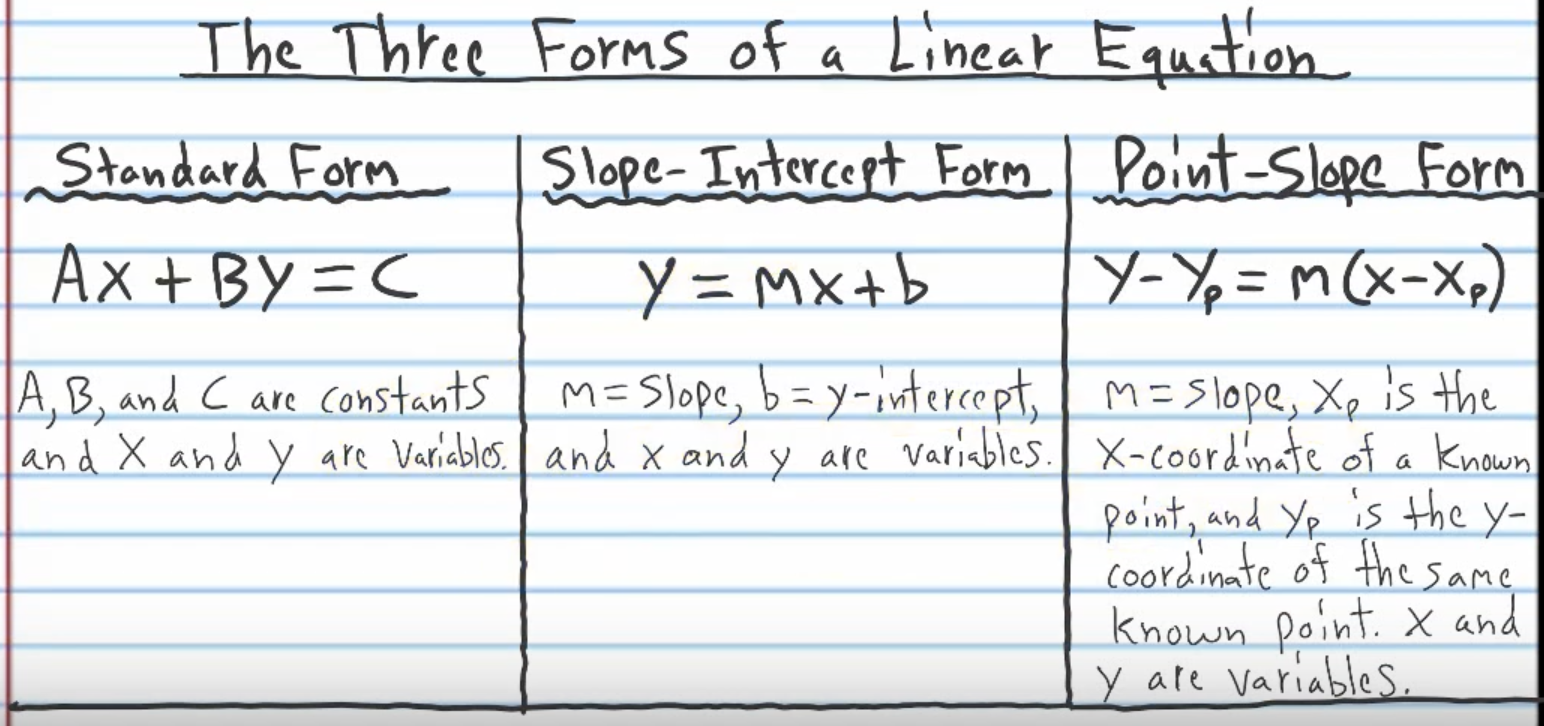
\includegraphics[width=1\textwidth]{beg2601.png}
  \caption{The Three Forms of a Linear Equation}
\end{figure}

% \par\rule{\textwidth}{0.5pt}

\textbf{Excercise}: Identify the form of each linear equation below by writing \q{S} for Standard, \q{SI} for slope-intercept, or \q{PS} for point-slope.

$2x+4y=3$: \textbf{S} because the variables x and y are on the same side of the equation.

$4=-8x+7x$: still Standard form, even though the equation is flipped.

$y-4=-3(x-5)$: \textbf{PS}, it is the only form that has parenthesses.

$y=2x+4$: \textbf{SI}, because the y is isolated on one side of the equation.

% \par\rule{\textwidth}{0.5pt}

\vspace{1 cm}

The standard form is not really useful for graphing. Nó không cho biết point, slope or y-intercept. Khi nhìn thấy standard form (x and y on the same side), convert into slope-Intercept form (where y is isolated). Slope-Intercept is the most useful form of the linear equation. Nó cho mình biết slope \& y-intercept.

You also need to be able to convert from Point-slope form to Slope-intercept form. Cách làm cũng là isolate y về một bên.

homework: 3

% Below is not from the course

\vspace{2 cm}

\textbf{Q:} Graph this line \(3x-4y=-6\)

Find the \textbf{x-intercept} by making y = 0. Then find the \textbf{y-intercept} by making x = 0.

\vspace{5mm}

\textbf{Q:} Graph this inequality \(y < -\frac{1}{3}x+2\)

Tìm tọa độ 2 điểm; vẽ đường thẳng.

\begin{itemize}
  \item Nếu \(\le\) thì vẽ straight line and shade under the line.
  \item Nếu > thì vẽ dashed line and shade above the line.
\end{itemize}

\textbf{Q: }Graphing Systems of Inequalities

\vspace{5mm}

Tính \textbf{Distance between 2 points} bằng Eq \ref{eq:3.2} below:

\begin{equation}
  d = \sqrt{(x_{1}-x_{2})^{2} + (y_{1}-y_{2})^{2}}
  \label{eq:3.2}
\end{equation}

\section{Graphing Linear Equations}

\hl{Method 01}: Finding two random points.

\hl{Method 02}: Finding x and y intercepts. Làm giống method 01 nhưng must chose $x=0$ and $y=0$. Useful when dealing with standard form.

\vspace{4cm}

\hl{Method 03}: Convert to Slope-Intercept form and use slope and y-intercept.

The slope is $\frac{\text{rise}}{\text{run}}$. In the figure below, first we find that the y-intercept is $(0,-1)$. Then we rise up two and run to the right 3 to get to the second point of $(3,1)$.

\begin{figure}[htb!]
  \centering
  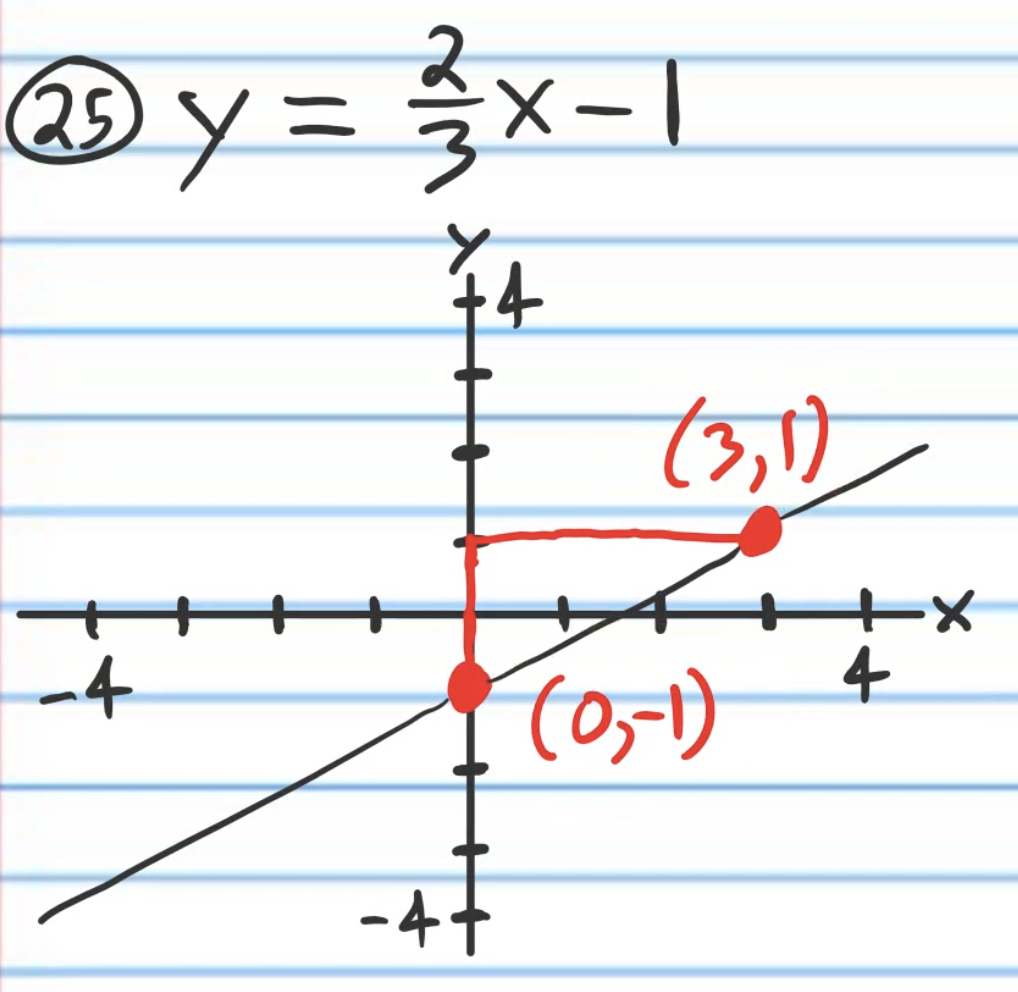
\includegraphics[width=0.6\textwidth]{beg2701.png}
  \caption{The slope is rise/run}
\end{figure}

When the slope is a negative number, instead of rising up, we go down and to the right. In the figure below, we go down 4 and then go 5 to the right (một ô đơn vị ứng với 2 units).

\begin{figure}[htb!]
  \centering
  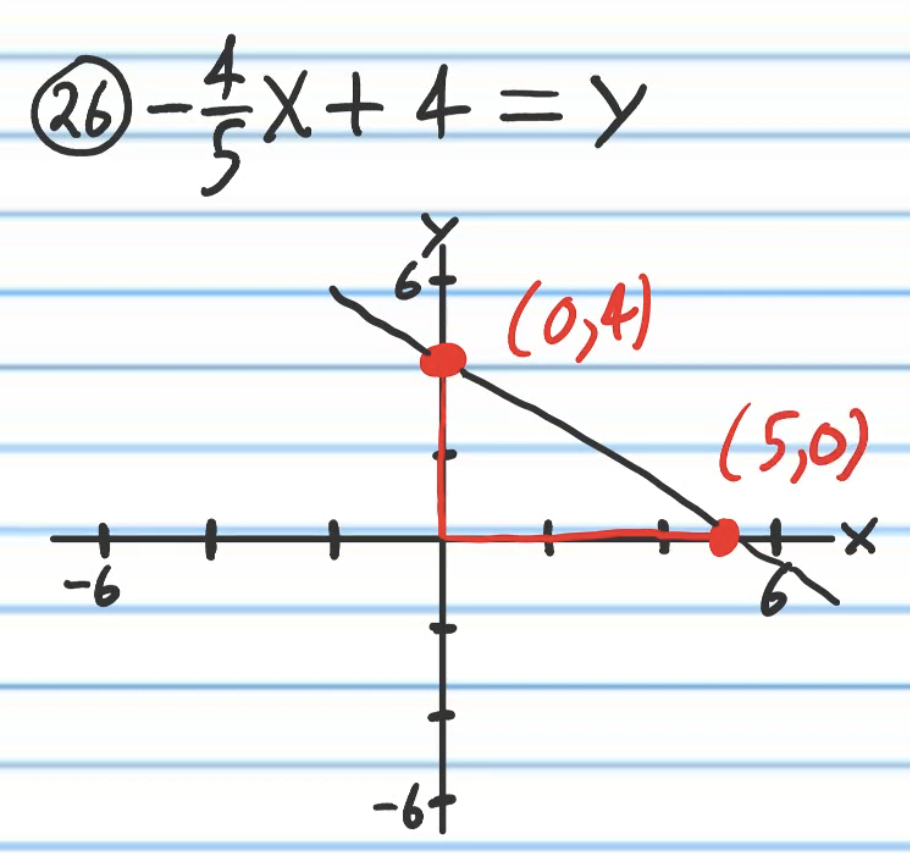
\includegraphics[width=0.6\textwidth]{beg2702.png}
  \caption{When the slope is negative}
\end{figure}

\vspace{1cm}

Nếu slope là whole number $2=\frac{2}{1}$. So rise 2 and run 1.

\vspace{1cm}

Nếu rise \& run chạy ra ngoài hệ trục mình vẽ như trong hình dưới nếu rise 5 and run 3 to the right thì outside the window. Vậy mình sẽ go \textbf{down} 5 and go 3 \textbf{to the left}. Nếu gặp negative slope thì revert bằng cách go up and to the left.

\begin{figure}[htb!]
  \centering
  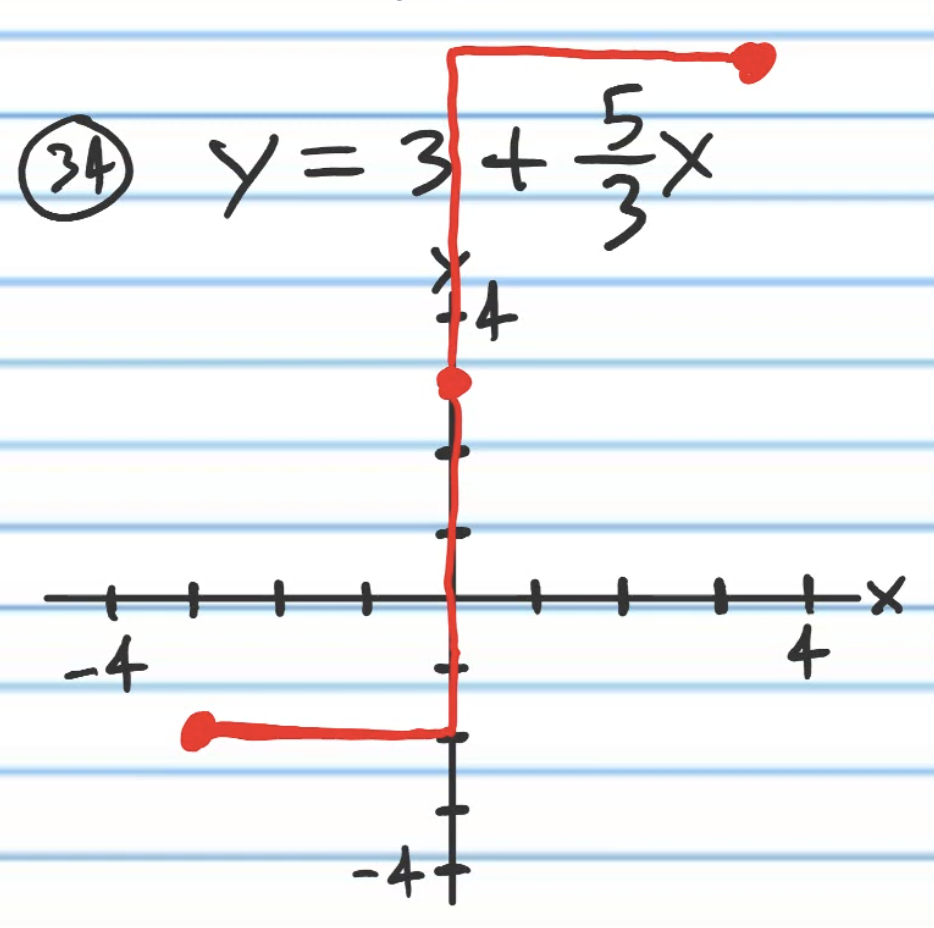
\includegraphics[width=0.6\textwidth]{beg2703.png}
  \caption{Go down and to the left}
\end{figure}

\hl{Method 04}: Using Point-Slope Form. Giống method 03.

\vspace{8mm}

In the problem below, kể cả khi revert the point thì vẫn ra ngoài our drawing window. Vậy thay vì go 3 and 4 whole units of one, we go 3 and 4 half-units of one (tức $\frac{1}{2}$) hoặc 3 and 4 third-units of one ($\frac{1}{3}$. The picture on the right go up three thirds (which is one whole $\frac{3}{3}=1$) and to the left four thirds $\frac{4}{3}$ to get to the x-coordinate $-(2+\frac{4}{3})=-3\frac{1}{3}$ (a mixed number). Chia một unit ra làm 3 phần bằng nhau. Nếu vẫn không đủ nữa thì chia ra fifths.

\begin{figure}[htb!]
  \centering
  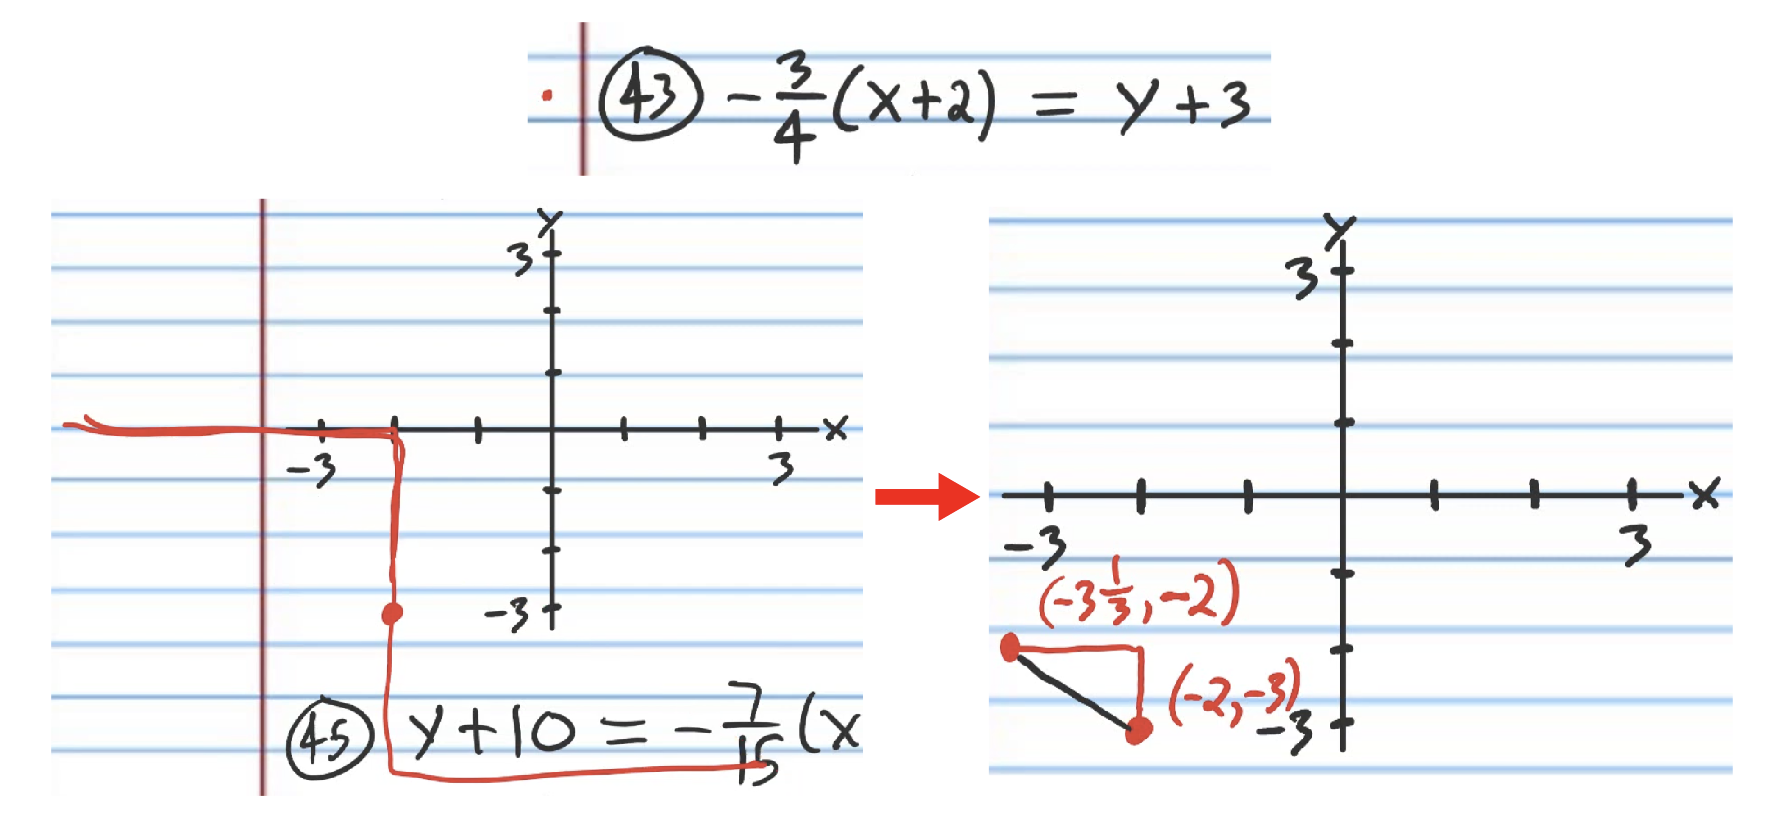
\includegraphics[width=0.9\textwidth]{beg2704.png}
  \caption{Go three thirds}
\end{figure}

\section{Additional Problems on Linear Equations and their Graphs}

